\documentclass[12pt]{article}
\usepackage[margin=2.5cm]{geometry}
\usepackage{enumerate}
\usepackage{amsfonts}
\usepackage{amsmath}
\usepackage{fancyhdr}
\usepackage{amsmath}
\usepackage{amssymb}
\usepackage{amsthm}
\usepackage{mdframed}
\usepackage{graphicx}
\usepackage{subcaption}
\usepackage{adjustbox}
\usepackage{listings}
\usepackage{xcolor}
\usepackage{booktabs}
\usepackage[utf]{kotex}
\usepackage{hyperref}
\usepackage{accents}

\definecolor{codegreen}{rgb}{0,0.6,0}
\definecolor{codegray}{rgb}{0.5,0.5,0.5}
\definecolor{codepurple}{rgb}{0.58,0,0.82}
\definecolor{backcolour}{rgb}{0.95,0.95,0.92}

\lstdefinestyle{mystyle}{
    backgroundcolor=\color{backcolour},
    commentstyle=\color{codegreen},
    keywordstyle=\color{magenta},
    numberstyle=\tiny\color{codegray},
    stringstyle=\color{codepurple},
    basicstyle=\ttfamily\footnotesize,
    breakatwhitespace=false,
    breaklines=true,
    captionpos=b,
    keepspaces=true,
    numbers=left,
    numbersep=5pt,
    showspaces=false,
    showstringspaces=false,
    showtabs=false,
    tabsize=1
}

\lstset{style=mystyle}

\pagestyle{fancy}
\renewcommand{\headrulewidth}{0.4pt}
\lhead{CSC 343}
\rhead{Topik II 2019 Reading Test Solution}

\begin{document}
\title{Topik II 2019 Reading Test Solution}
\maketitle

\begin{enumerate}[1.]
    \item ※ [1~2] (   )에 들어갈 가장 알맞은 것을 고르십시오. (각 2점)

    \bigskip

    1. 나는 주말에는 보통 영화를 (       ) 운동을 한다.

    \bigskip

    \begin{enumerate}[1)]
        \item 보지만
        \item 보거나
        \item 보려고
        \item 보더니
    \end{enumerate}

    \bigskip

    \textbf{Answer:} 2
    \item
    \item 4
    \item 4
    \item 1
    \item 2
    \item 4
    \item 1
    \item 3
    \item 1
    \item 4
\end{enumerate}

※ [1~2] (   )에 들어갈 가장 알맞은 것을 고르십시오. (각 2점)

\begin{enumerate}[1.]
    \item 나는 주말에는 보통 영화를 (       ) 운동을 한다.

    \begin{enumerate}[1)]
        \item 보지만
        \item 보거나
        \item 보려고
        \item 보더니
    \end{enumerate}

    \item 동생이 점점 아버지를 (       ).

    \begin{enumerate}[1)]
        \item 닮아 간다
        \item 닮기도 한다
        \item 닮았나 보다
        \item 닮은 적이 없다
    \end{enumerate}


    \item ※ [3~4] 다음 밑줄 친 부분과 의미가 비슷한 것을 고르십시오. (각 2점)

    \bigskip

    정부는 일자리를 늘리고자 새로운 정책을 수립했다.

    \begin{enumerate}[1)]
        \item 늘리자마자
        \item 늘리더라도
        \item 늘리는 대신
        \item 늘리기 위해
    \end{enumerate}


    \item 태어난 지 얼마 안 되어 서울로 왔으니 서울이 고향인 셈이다.

    \begin{enumerate}[1)]
        \item 고향일 뿐이다
        \item 고향이면 좋겠다
        \item 고향일 리가 없다
        \item 고향이나 마찬가지이다
    \end{enumerate}




    \item [5~8] 다음은 무엇에 대한 글인지 고르십시오. (각 2점)

    \begin{center}
    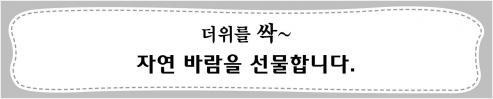
\includegraphics[width=0.7\linewidth]{images/2019_1.png}
    \end{center}


    \begin{enumerate}[1)]
        \item 에어컨
        \item 청소기
        \item 냉장고
        \item 세탁기
    \end{enumerate}


    \item

    \begin{center}
    \includegraphics[width=0.7\linewidth]{images/2019_2.png}
    \end{center}

    \begin{enumerate}[1)]
        \item 병원
        \item 은행
        \item 여행사
        \item 체육관
    \end{enumerate}


    \item

    \begin{center}
    \includegraphics[width=0.7\linewidth]{images/2019_3.png}
    \end{center}

    \bigskip

    \begin{enumerate}[1)]

        \item 건강 관리
        \item 화재 예방
        \item 이웃 사랑
        \item 환경 보호
    \end{enumerate}


    \item

    \begin{center}
    \includegraphics[width=0.7\linewidth]{images/2019_4.png}
    \end{center}

    \begin{enumerate}[1)]
        \item 이용 안내
        \item 구입 문의
        \item 사용 순서
        \item 교환 방법
    \end{enumerate}




    \item ※ [9~12] 다음 글 또는 그래프의 내용과 같은 것을 고르십시오. (각 2점)

    \begin{center}
    \includegraphics[width=0.7\linewidth]{images/2019_5.png}
    \end{center}

    \begin{enumerate}[1)]
        \item 이 대회는 이번에 처음으로 열린다.
        \item 이 대회에는 누구나 참가할 수 있다.
        \item 이 대회에 참가하려면 돈을 내야 한다.
        \item 이 대회의 출발 장소는 인주기념관이다.
    \end{enumerate}

    \item

    \begin{center}
    \includegraphics[width=0.7\linewidth]{images/2019_6.png}
    \end{center}

    \begin{enumerate}[1)]
        \item 1위 순위의 직업이 바뀌었다.
        \item 공무원은 순위의 변화가 없었다.
        \item 군인이 새롭게 5위 안에 들었다.
        \item 간호사는 4위로 순위가 떨어졌다.
    \end{enumerate}


    \item

    \begin{mdframed}

    지난 24일에 ‘제7회 소비자 선정 최고 브랜드 대상’ 시상식이 인주신문사
    대강당에서 개최됐다. 이 상은 소비자의 온라인 투표로 수상 브랜드가
    선정되어 의미가 크다. 지난해와 같이 100개 브랜드가 상을 받았는데 올해는
    처음으로 친환경 화장품 브랜드 두 개가 포함되었다.

    \end{mdframed}

    \begin{enumerate}[1)]
        \item 소비자가 수상 브랜드를 선정했다.
        \item 기업들이 직접 온라인 투표에 참여했다.
        \item 지난해보다 더 많은 브랜드가 선정됐다.
        \item 친환경 화장품 브랜드는 상을 못 받았다.
    \end{enumerate}


    \item

    \begin{mdframed}

    최근 한 나라에서 4,400년 전에 만들어진 무덤이 발견됐다. 이 무덤의

    주인은 당시 왕으로 밝혀졌으며 무덤 벽에는 고대 문자와 다양한 색의

    그림이 가득했다. 이 무덤은 오랜 시간이 지났지만 색이 거의 그대로 보존

    되어 있어 역사적 가치가 높다고 전문가들은 전했다. 무덤의 일부는 일반인

    에게도 곧 공개될 예정이다.

    \end{mdframed}

    \begin{enumerate}[1)]
        \item 무덤의 주인이 누구인지 찾고 있다.
        \item 무덤 안을 구경하는 사람들이 많아졌다.
        \item 무덤 안의 그림은 색의 상태가 좋은 편이다.
        \item 무덤 바닥에서 다양한 문자와 그림이 발견됐다.
    \end{enumerate}




    \item [13~15] 다음을 순서대로 맞게 배열한 것을 고르십시오. (각 2점)

    \begin{mdframed}
    (가) 회사의 1층 로비를 외부인에게 개방하는 회사가 많아졌다.

    (나) 사람들은 작품을 감상하고 커피를 마시면서 시간을 보낸다.

    (다) 미술관과 카페를 만들어 사람들이 와서 즐길 수 있게 한 것이다.

    (라) 이 공간을 이용하는 사람이 늘면서 회사의 이미지도 좋아지고 있다.
    \end{mdframed}

    \begin{enumerate}[1)]
        \item (가)-(다)-(나)-(라)
        \item (나)-(라)-(다)-(가)
        \item (다)-(나)-(라)-(가)
        \item (라)-(나)-(가)-(다)
    \end{enumerate}


    \item
    \begin{mdframed}
    (가) 차에서 내려 앞차의 주인에게 사과하고 사정을 설명했다.

    (나) 앞차 주인은 큰 사고가 아니니 괜찮다며 그냥 가라고 했다.

    (다) 친절한 배려 덕분에 딸은 무사히 병원에 도착해 치료를 받았다.

    (라) 아픈 딸을 병원으로 급하게 데려가다가 앞차와 부딪쳐서 사고를 냈다.
    \end{mdframed}

    \begin{enumerate}[1)]
        \item (나) - (가) - (다) - (라)
        \item (나) - (가) - (라) - (다)
        \item (라) - (가) - (나) - (다)
        \item (라) - (가) - (다) - (나)
    \end{enumerate}


    \item

    \begin{mdframed}
    (가) 선택에 대한 부담으로 구매를 망설이다가 포기하기도 한다.

    (나) 선택에 대한 고객의 부담을 줄여 구매를 유도하려는 것이다.

    (다) 그래서 마트에서는 품목별로 몇 가지의 제품만 매장에 진열한다.

    (라) 소비자는 선택의 폭이 넓을수록 물건을 고를 때 어려움을 겪는다.
    \end{mdframed}

    \begin{enumerate}[1)]
        \item (나)-(가)-(라)-(다)
        \item (나)-(라)-(가)-(다)
        \item (라)-(가)-(다)-(나)
        \item (라)-(다)-(가)-(나)
    \end{enumerate}




    \item ※ [16~18] 다음을 읽고 (   )에 들어갈 내용으로 가장 알맞은 것을 고르십시오. (각 2점)


    \begin{mdframed}
    상담을 통해 책을 추천해 주는 서점이 있어 화제가 되고 있다. 서점

    주인은 손님과 오랜 시간 대화를 나눈 후 (     ) 책을 추천해

    준다. 상처 받은 사람에게는 위로가 되는 책을,자신감이 부족한 사람에게는

    용기를 주는 책을 추천하는 방식으로 서비스를 제공한다.
    \end{mdframed}

    \begin{enumerate}[1)]
        \item 내용이 재미있는
        \item 지식을 전달하는
        \item 사람들이 많이 읽는
        \item 손님의 상황에 맞는
    \end{enumerate}


    \item

    \begin{mdframed}
    샌드위치나 샐러드 등은 오래 보관할 수 없어 신선할 때 팔아야 한다.

    이런 식품을 영업 마감 시간을 앞두고 사람들에게 할인된 가격으로 판매

    하는 서비스가 큰 호응을 얻고 있다. 음식점은 남은 음식을 팔아 수익을

    얻을 수 있고,소비자는 (     ) 이용자들의 만족도가 높다.

    \end{mdframed}

    \begin{enumerate}[1)]
        \item 자원을 아낄 수 있어서
        \item 식품을 저렴하게 살 수 있어서
        \item 요리법을 배울 수 있기 때문에
        \item 음식을 선택할 수 있기 때문에
    \end{enumerate}


    \item

    \begin{mdframed}
    뮤지컬은 보통 한 역할에 여러 명의 배우들이 출연한다. 배우에 따라
    연기나 분위기가 다르기 때문에 같은 작품이라도 색다른 느낌을 받을 수
    있다 그래서 뮤지컬 팬들은 (      ) 작품을 즐기기 위해 공연을
    반복해서 관람한다.
    \end{mdframed}

    \begin{enumerate}[1)]
        \item 입장료를 할인해 주는
        \item 공연장에서 인기가 있는
        \item 유행하는 노래가 나오는
        \item 각 배우들의 개성이 담긴
    \end{enumerate}



    \item ※ [19~20] 다음을 읽고 물음에 답하십시오. (각 2점)

    \begin{mdframed}
    해파리는 몸의 95\%가 물로 구성되어 있어 열량이 낮다. 그래서 해파리를

    먹고 사는 동물이 거의 없다고 알려져 있었다. 하지만 새나 팽귄,뱀장어

    등 많은 동물들에게 해파리는 좋은 먹잇감이다. 해파리에는 비타민이나

    콜라겐 같은 영양 성분이 있기 때문이다. (      ) 해파리는 바다 어디에나

    있고 도망치지 않아 사냥하기 쉽기 때문이다.
    \end{mdframed}

    \bigskip

    (   )에 들어갈 알맞은 것을 고르십시오.

    \bigskip

    \begin{enumerate}[1)]
        \item 과연
        \item 만약
        \item 게다가
        \item 이처럼
    \end{enumerate}


    \item 위 글의 내용과 같은 것을 고르십시오.

    \begin{enumerate}[1)]
        \item 해파리는 바다 생태계에 피해를 준다.
        \item 해파리는 잡기 어려운 먹이 자원이다.
        \item 해파리는 여러 동물의 먹이가 되고 있다.
        \item 해파리는 대부분 콜라겐으로 이루어져 있다.
    \end{enumerate}



    \item ※ [21~22] 다음을 읽고 물음에 답하십시오. (각 2점)

    \begin{mdframed}
    내비게이션은 목적지까지 길을 안내해 주는 기기이다. 내비게이션이

    없이 낯선 곳에 갔다가 길을 못 찾아 (    ) 본 적이 있는

    사람이라면 내비게이션이 얼마나 편리한지 느꼈을 것이다. 그러나 우리의

    뇌는 스스로 정보를 찾았을 때 그 정보를 오래 기억하는 특성이 있다.

    따라서 지나치게 디지털 기기에만 의존하다 보면 정보를 찾고 기억하는

    능력이 점점 줄어들어 결국 그 능력을 사용할 수 없게 될지도 모른다.
    \end{mdframed}

    \bigskip

    (   )에 들어갈 알맞은 것을 고르십시오.

    \bigskip

    \begin{enumerate}[1)]
        \item 앞뒤를 재어
        \item 진땀을 흘려
        \item 발목을 잡아
        \item 귀를 기울여
    \end{enumerate}

    \item 위 글의 중심 생각을 고르십시오.

    \begin{enumerate}[1)]
        \item 디지털 기기는 편리한 생활을 위해 필요하다.
        \item 운전자에게 내비게이션은 활용도가 매우 높다.
        \item 스스로 정보를 찾고 기억하려는 노력을 해야 한다.
        \item 내비게이션을 잘 활용하면 기억력 향상에 도움이 된다.
    \end{enumerate}



    \item [23~24] 다음 글을 읽고 물음에 답하십시오. (각 2점)

    \begin{mdframed}
    놀이공원 매표소에서 아르바이트를 했다. 아르바이트가 처음이라 실수를

    하지 않으려고 늘 긴장하면서 일을 했다. 어느 날,놀러 온 한 가족에게

    인원수만큼 표를 줬다. 그런데 그 가족을 보내고 나서 이용권 한 장의 값이

    더 결제된 것을 알아차렸다. 바로 카드사로 전화해 고객의 전화번호를

    물었지만 상담원은 알려 줄 수 없다고 했다. 하지만 내 연락처를 고객에게

    전달해 주겠다고 했다. 일을 하는 내내 일이 손에 잡히지 않았다. 퇴근

    시간 무렵 드디어 그 가족에게서 전화가 왔다. 내가 한 실수에 화를 낼지도

    모른다는 생각에 떨리는 목소리로 상황을 설명하자 그 가족은 “놀이 기구를

    타고 노느라 문자 메시지가 온 줄 몰랐어요. 많이 기다렸겠어요.”라고 하며

    따뜻하게 말해 주었다.
    \end{mdframed}

    \bigskip

    밑줄 부분에 나타난 ‘나’의 심정으로 알맞은 것을 고르십시오.

    \bigskip

    \begin{enumerate}[1)]
        \item 걱정스럽다
        \item 불만스럽다
        \item 후회스럽다
        \item 당황스럽다
    \end{enumerate}


    \item 위 글의 내용과 같은 것을 고르십시오.

    \begin{enumerate}[1)]
        \item 그 가족은 나에게 화를 냈다.
        \item 카드 회사는 그 가족에게 연락을 했다.
        \item 나는 그 가족에게 직접 전화를 걸었다.
        \item 나는 그 가족을 찾아다니느라 일을 못 했다.
    \end{enumerate}



    \item ※ [25~27] 다음 신문 기사의 제목을 가장 잘 설명한 것을 고르십시오. (각 2점)

    \bigskip

    관광버스 추락,안전벨트로 승객 전원 목숨 건져

    \bigskip

    \begin{enumerate}[1)]
        \item 관광버스가 추락했지만 승객들이 안전벨트 덕분에 모두 살았다.
        \item 관광버스 추락 사고 이후 안전벨트를 하는 승객이 더 많아졌다.
        \item 관광버스가 추락하자 일부 승객이 안전벨트를 풀고 탈출하였다.
        \item 관광버스가 추락하면서 안전벨트를 한 일부 승객이 크게 다쳤다.
    \end{enumerate}


    \item 침묵 깬 김민수 의원,대통령 선거 출마설 부인

    \begin{enumerate}[1)]
        \item 김 의원이 대통령 선거에 나가느냐는 질문에 계속 답하지 않고 있다.
        \item 김 의원이 마음을 바꾸어 대통령 선거에 나가겠다고 최종 발표하였다.
        \item 김 의원이 대통령 선거에 나간다고 선언하자 사람들이 열렬히 환영했다.
        \item 김 의원이 대통령 선거에 나간다는 것이 사실이 아니라고 입장을 밝혔다.
    \end{enumerate}



    \item 민간 우주선 무사 귀환,우주여행 시대 ‘성큼’

    \begin{enumerate}[1)]
        \item 사람들의 응원 속에 민간 우주선이 긴 우주여행을 마치고 돌아왔다.
        \item 사람들은 민간 우주선이 우주여행에서 무사히 돌아오기를 기대했다.
        \item 민간 우주선이 무사히 돌아오면서 우주여행의 가능성이 더욱 높아졌다.
        \item 민간 우주선이 돌아오지 않자 우주여행에 대한 우려의 목소리가 커졌다.
    \end{enumerate}


    \item ※ [28~31] 다음을 읽고 (   )에 들어갈 내용으로 가장 알맞은 것을 고르십시오. (각 2점)


    \begin{mdframed}
    새해에 세운 목표를 효과적으로 이루려면 한 주 단위로 계획을 세우는

    것이 좋다. 주마다 계획을 세우면 (     )때문이다. ‘건강한

    식습관 기르기’라는 새해 결심이 한 주 단위가 되면 ‘라면 안 먹기’,'채소

    챙겨 먹기’처럼 구체적인 계획으로 바뀐다. 이렇게 하면 작은 목표를 달성

    하는 횟수가 늘어 한 해의 목표에 가까워진다.
    \end{mdframed}

    \begin{enumerate}[1)]
        \item 한 해의 목표를 확인하기
        \item 계획을 세우는 데 집중하기
        \item 자신의 능력을 보여 줄 수 있기
        \item 실천 가능한 계획을 세울 수 있기
    \end{enumerate}


    \item

    \begin{mdframed}
    무지개는 빛이 공기중의 물방울을 통과할 때 굴절되어 나타나는

    현상이다. 그래서 비가 그친 직후 해가 뜰 때 무지개가 잘 생긴다. 이때

    (      ) 않으면 무지개가 만들어지기 어렵다. 공기에 먼지 등의

    오염 물질이 섞이면 물방울들이 먼지 주위로 모여 빛이 통과하는 것을

    막기 때문이다.
    \end{mdframed}

    \begin{enumerate}[1)]
        \item 해가 뜨지
        \item 비가 그치지
        \item 빛이 약하지
        \item 공기가 깨끗하지
    \end{enumerate}


30.
  취재 경계선은 취재가 과열되어 발생할 수 있는 불상사를 예방하기
위해 설정한 것이다. 수백 명의 취재진이 화제의 인물에게 몰려들 경우
사고가 발생해 취재를 망칠 수 있다. 그래서 선을 그어 놓고 그 바깥에서
취재하자는 합의를 본 것이다. 비록 법으로 정해져 있지 않지만 언론계가
이 선을 지키려고 노력하는 것은 (      ) 순간 원활한 보도가
어려워진다는 것을 누구보다 잘 알고 있기 때문이다.
① 취재 정보를 공유하는
② 취재 경계선이 무너지는
③ 취재 내용을 잘못 해석하는
④ 취재 경계선이 새로 설정되는


31.
  병원의 규모에 따라 개인이 부담해야 하는 약값을 달리하는 제도가
생겼다. 감기와 같이 비교적 가벼운 병에 걸렸을 때 종합병원에서 진료를
받으면 (      ) 만든 것이다. 같은 약을 동네 의원에서 받은
처방전으로 사게 되면 약값이 더 적게 나온다. 이 제도를 통해 환자들이
진료에 대한 신뢰 때문에 종합병원으로만 몰리는 현상을 줄일 수 있을
것으로 예상된다.
① 환자가 약값을 조금 더 내게
② 개인이 약값을 비교할 수 있게
③ 병원에서 병원비를 올리지 못하게
④ 병원비의 일부를 병원에서 지원하게




※ [32~34] 다음을 읽고 내용이 같은 것을 고르십시오. (각 2점)

32.
  나비 박사 석주명은 나비의 종류를 분류하고 이름을 지어 준 생물학자
이다. 1931년부터 나비를 연구한 그는 한국의 나비가 총 844종이라는 당시의
분류를 248종으로 수정하였다. 날개 무늬나 모양이 조금만 달라도 다른
종이라고 판단한 기존의 분류가 틀렸음을 배추흰나비 16만여 마리의 무늬를
비교해서 밝혔다. 또한 그때까지 한자어나 외래어로 명명된 나비에 ‘떠들썩
팔랑나비’와 같은 고유어 이름을 지어 주는 데 앞장섰다.
① 석주명은 한국의 나비를 총 844종으로 분류하였다.
② 석주명은 나비 이름을 고유어로 바꾸려고 노력하였다.
③ 석주명은 자신의 배추흰나비 연구에 문제가 있음을 알았다.
④ 석주명은 나비의 날개 모양이 다르면 종이 달라짐을 밝혔다.


33.
  저축의 방식을 가로 저축과 세로 저축으로 나눠 비유하여 설명할 수
있다. 차량 구입이나 주택 마련과 같이 특정 목적을 위해 한 통장에 집중하여
저축하는 것이 세로 저축이다. 반면 장기적으로 다양한 목적에 따라 자금을
여러 통장에 분산하여 저축하는 것을 가로 저축이라고 한다. 단기적으로
빨리 목돈을 만들고 싶다면 세로 저축을,은퇴 후의 생활까지 고려한다면
가로 저축을 선택하는 것이 좋다.
① 노후 준비에는 세로 저축이 유리하다.
② 세로 저축보다 가로 저축을 하는 것이 더 좋다.
③ 저축의 목적이 다양하면 가로 저축이 유용하다.
④ 가로 저축은 단기적인 계획이 있을 때 효율적이다.


34.
  '책가도’는 책장과 책을 중심으로 하여 각종 문방구 등을 그린 그림이다.
학문을 중요시하는 왕의 바람과 출세를 원하는 양반의 마음이 더해져
책가도는 궁중과 사대부를 중심으로 발전하였다. 19세기에는 상인과 농민
계층으로도 확산되면서 그 형식도 자유로워졌다. 그림에서 책장 대신 작은
탁자가 활용되기도 하고 일상 용품이 함께 그려지기도 했다.
① 왕은 책가도에 대해 부정적 인식이 강했다.
② 점차 다양한 계층에서 책가도를 즐기게 되었다.
③ 초기의 책가도에는 일상 용품이 주로 그려졌다.
④ 책가도는 왕의 바람으로 그림의 형식이 바뀌었다.




※ [35~38] 다음 글의 주제로 가장 알맞은 것을 고르십시오. (각 2점)

35.
  문화재 복원 작업은 복원된 부분이 자연스러워야 하고 그 과정에서
문화재가 추가로 손상되지 않아야 한다. 이 때문에 정확한 측정으로 복원할
부분을 원래 모습과 동일하게 만들어 내는 것은 복원의 성공을 결정하는
중요한 요건이다. 최근 3D 스캐너와 프린터가 등장하여 이러한 요건을
충족할 수 있게 되면서 정밀하고 안전한 문화재 복원이 가능해졌다.
① 첨단 장비 덕분에 문화재 복원이 수월해졌다.
② 문화재는 손상 예방을 위한 사전 관리가 중요하다.
③ 복원 환경 탓에 원본이 변형되는 경우가 많아지고 있다.
④ 복원 기술자를 대상으로 한 3D 장치 사용 교육이 필요하다.


36.
  아기는 주변 사물을 손으로 더듬고 만지면서 지각 능력을 발달시킨다.
그런데 이렇게 능동적인 경험뿐만 아니라 사람,햇빛,바람 등에 의한 접촉도
주요한 촉각 경험이 된다. 그중 주변 인물과의 피부 접촉은 사랑,유대감,
신뢰감 등 유아의 정서 발달과 사회성 발달에 매우 중요하다. 연구에 따르면
아기가 태어난 후 몇 년 사이에 이루어진 피부 접촉은 정서 발달에 필수적인
호르몬 분비를 촉진할 뿐만 아니라 지능 발달에도 영향을 미친다고 한다.
① 인간은 촉각을 통해 주변 사물을 이해한다.
② 정서 발달과 지능 발달은 상관관계가 높다.
③ 촉각 경험의 중요성에 대한 연구가 필요하다.
④ 유아의 발달을 위해서는 피부 접촉이 중요하다.


37.
  나무에 붙어 자라는 버섯을 보면 나무로부터 양분을 받으며 별다른 노력
없이 살아간다고 생각하기 쉽다. 하지만 버섯은 나무에게 없어서는 안 될
중요한 존재이다. 나무들은 위기 상황이 발생해도 자리를 옮겨 이를 알릴
수 없기 때문에 뿌리로 소통하며 위험에 대비한다. 이때 뿌리가 짧아 서로
닿지 않는 나무들 사이에서는 실처럼 뻗은 버섯 균사체가 메시지 전달을
대신한다. 그래서 학자들은 버섯 균류를 ‘숲의 통신망’이라고 부른다.
① 버섯은 다른 식물이 있어야 자랄 수 있다.
② 나무의 뿌리가 숲에서 하는 기능은 다양하다.
③ 버섯은 숲에서 나무들의 정보 교환을 돕는 역할을 한다.
④ 나무의 생활환경에 대한 학자들의 관심이 높아지고 있다.


38.
  음주 운전으로 인명 피해를 낸 사람에 대한 처벌 강화 법안이 국회에서
통과되었다. 하지만 새 법안은 원래 안건보다 처벌의 강도를 낮춘 것이라는
점에서 반쪽짜리 법안에 불과하다. 이 법안에 따르면 여전히 음주 운전
가해자의 처벌이 미뤄지거나 일정 기간이 지난 후 효력이 없어질 수도
있다. 이는 음주 운전에 대한 경각심을 높이고 재발 위험성을 낮추려던
본래의 취지에는 맞지 않는 것이다.
① 법안이 가진 본래의 취지를 널리 알려야 한다.
② 피해 정도에 따라 처벌의 수위를 조절해야 한다.
③ 새 법안의 통과가 더 이상 미루어져서는 안 된다.
④ 새 법안은 실질적 효과를 거두는 데 미흡한 점이 있다.




※ [39~41] 다음 글에서 <보기>의 문장이 들어가기에 가장 알맞은 곳을 고르십시오. (각 2점)

39.
  왕관은 과거 지배 계층이 착용했던 대표적인 장신구이다.( ㉠ ) 장식도
화려하게 더해져 그것을 쓴 왕의 지위를 더욱 돋보이게 했다. ( ㉡ )
오늘날 왕관이 가졌던 힘과 지위의 의미는 약화되었으나 고귀한 이미지는
남아 여러 디자인에서 발견된다 ( ㉢ ) 아름다움이 강조되어야 할 신부의
머리 장식이나 여러 액세서리에 왕관이 활용되고 있는 것이다. ( ㉣ )

<보 기>

그래서 백성들이 구하기 힘든 매우 귀하고 값비싼 재료로 만들어졌다.
① ㉠	② ㉡	③ ㉢	④ ㉣


40.
  멸종 위기에 처한 동물을 보호하려는 노력이 계속되고 있으나 주된 연구와
지원이 몇몇 동물에 쓸리고 있어 문제가 되고 있다.( ㉠ ) 한 조사에
따르면 동물 보호 기금의 모금 액수도 북극곰,판다같이 인기 있는 동물들
에게 편중되었다고 한다. ( ㉡ ) 이런 가운데 그간 관심을 받지 못했던
동물들을 보호하기 위한 단체가 등장했다. ( ㉢ ) 이러한 노력은 동물
보호를 위한 마음에도 편견이 깃들어 있었음을 일깨우고 있다. ( ㉣ )

<보 기>

그들은 못생기고 혐오감을 준다는 이유만으로 외면당한 동물들을 대중에게
알리는 활동을 한다.
① ㉠	② ㉡	③ ㉢	④ ㉣


41.
  ‘젊은 작가상’을 수상한 최은영이 두 번째 소설집『내게 무해한 사람』을
펴냈다. ( ㉠ ) 2년여에 걸쳐 여러 지면에 발표했던 작품들을 한 권에
모은 것이다. ( ㉡ ) 그들처럼 누군가에 대한 배반,원치 않았던 이별 등
매듭짓지 못한 일들을 다시 떠올린다는 것은 괴로운 과정일 것이다.
( ㉢ ) 그러나 작가는 이미 지나간 시간에 대해 후회할 필요는 없으며
상처도 힘이 될 수 있다는 메시지로 독자의 마음을 움직인다. ( ㉣ )

<보 기>

일곱 편의 단편에는 오해와 잘못으로 멀어진 사람들에 대한 이야기가
담겨 있다.
① ㉠	② ㉡	③ ㉢	④ ㉣




※ [42~43] 다음을 읽고 물음에 답하십시오. (각 2점)

  그때 소희네는 이사를 앞두고 있었는데 엄마는 그렇게 집을 나가 돌아
오지 않았다. 작별 인사는커녕 아무 신호도 낌새도 없이 휙 사라졌다. (중략)
엄마가 집 나가고 열흘쯤 지났을 땐가,소희가 텔레비전을 보고 있는데
본회가 현관에서 신을 신으며 잠깐 나갔다 오겠다고 했다.
  “잠깐 어디?” “친구네.” “친구 누구?” 소희가 눈을 맞추려 했지만 본희는
돌아보지 않았다.“늦으면 친구네서 자고 올지도 몰라. 기다리지 말고 자.”
돌아서 나가는 본희가 멘 가방이 이상하게 커 보여 소희는 자리에서 벌떡
일어났다. 가만히 서 있다가 갑자기 현관문을 열고 맨발로 뛰어나가 계단을
올라가는 본희 뒷모습에 대고 외쳤다.“언니야,올 거지?” 본희는 멈춰
섰지만 돌아보지 않았다. 소희는 묻고 또 물었다.(중략)
   한참 있다가,몇 년은 지난 거 같은데 몇 시간쯤밖에 안 지난 한밤중에
언니가 문자를 했다. 소희는 언니가 올 때까지 휴대 전화를 손에 꼭 쥐고
문자를 보고 또 보았다. 그러지 않으면 문자가 감쪽같이 날아갈 것 같았다.
   삼겹살 사가지고 가께. 라면 끓여먹지 말고 기다려.


42. 밑줄 친 부분에 나타난 '소희'의 심정으로 알맞은 것을 고르십시오.

① 불안하다	② 흡족하다
③ 실망스럽다	④ 감격스럽다


43. 위 글의 내용과 같은 것을 고르십시오.

① 본희는 밤늦게 소희에게 연락을 줬다.
② 엄마는 이사하는 날에 집으로 돌아왔다.
③ 본희는 소희를 데리고 친구 집에 놀러 갔다.
④ 소희는 엄마를 기다리며 휴대 전화를 놓지 못했다.




※ [44~45] 다음을 읽고 물음에 답하십시오. (각 2점)

  성대하고 까다로운 제사 준비 탓에 유교 예법을 비판하는 사람들이
많다. 하지만 현재 우리가 지키고 있는 예법은 (      ) 잘못된
예법이 전해져 온 것이다. 유교 전문가들은 제사든 차례든 조상을 공경하는
마음과 자손들의 화목이 중요하다고 말한다. 선조들은 제사를 드릴 때
좋은 음식을 많이 준비하는 것보다 그 음식을 준비하는 마음과 정성을
중시했던 것이다. 유서 깊은 집안에서는 이러한 제사의 본질을 제대로
이해하여 상차림은 간소하게 하되 집안사람들이 모두 모여 함께 제사를
드리는 경우가 많다. 형식보다 정성이 중요하다는 유교의 가르침을 지키고
있는 것이다.


44. 위 글의 주제로 알맞은 것을 고르십시오.

① 조상을 모시는 제사상 차림은 점차 간소화되고 있다.
② 유교 문화는 후손들에 의해 유동적으로 변화되고 있다.
③ 명절에 제사를 드리는 전통은 예법에 맞게 유지되고 있다.
④ 유교 예법에서 중요한 것은 정성을 다해 예를 갖추는 것이다.


45. (   )에 들어갈 내용으로 가장 알맞은 것을 고르십시오.

① 상차림이 간소화된
② 후손들의 바람이 반영된
③ 유교의 본뜻을 살리지 못한
④ 현실에 맞게 축소되지 않은




※ [46~47] 다음을 읽고 물음에 답하십시오. (각 2점)

  1인 미디어 시대가 되면서 개인 방송을 이용한 새로운 시장 형태가 등장해
주목받고 있다. 이 시장은 SNS를 통해 제품이 유통되고 판매된다는 특징이
있 다 . ( ㉠ ) 대표적인 판매방식은 1인 미디어 운영자가 방송 중에
특정 물건을 의도적으로 노출하여 구매를 유도하는 것이다. 이때 관심이
생긴 시청자는 그 운영자에게서 물건을 산다. ( ㉡ ) SNS 계정만
있으면 누구든지 판매를 시작할 수 있으며 제품 홍보부터 구매까지 모든
과정이 SNS상에서 이루어진다 ( ㉢ ) 덕분에 초기 사업 비용이 거의
들지 않는다는 장점이 있다. ( ㉣ ) 하지만 개별 사업자의 수가 무한
하게 늘 수 있기 때문에 향후 경제 변화를 이끌 핵심 시장으로의 성장이
예상된다.


46.
위 글에서 <보기>의 글이 들어가기에 가장 알맞은 것을 고르십시오.
<보 기>

이와 같은 시장 형태가 전체 소비 시장에 미치는 영향력은 아직 미미하다.
① ㉠	② ㉡	③ ㉢	④ ㉣


47. 위 글의 내용과 같은 것을 고르십시오.

① 1인 미디어 운영자는 이 시장의 운영에 참여할 수 없다.
② 이 시장의 운영자들은 시장 경제에 부정적인 영향을 미친다.
③ 1인 미디어 시청자는 방송을 보다가 제품을 구매할 수 있다.
④ 이 시장을 처음 시작할 때는 충분한 자본 투자가 필수적이다.




※ [48~50] 다음을 읽고 물음에 답하십시오. (각 2점)

  올해 ‘자치경찰제’가 전국으로 확대될 예정이다. 자치경찰제는 지방자치
단체가 경찰의 운영 및 관리를 담당하도록 하는 제도를 말한다. 이 제도가
실시되면 경찰이 지역 주민의 삶에 밀착돼 지역 특성에 맞는 다양한 서비
스를 주민들에게 제공할 수 있을 것으로 보인다. 그러나 제도적 취약점과
예측되는 부작용이 있을 수 있다. 무엇보다 현장에서의 혼선이 예상된다.
제도에 따르면 자치경찰은 교통사고나 가정 폭력 조사 등 생활 안전 부분을
담당하고 국가 보안이나 전국 단위의 수사는 지금처럼 국가경찰이 맡는다.
이처럼 경찰 조직이 이중 구조일 때 어려움을 겪는 것은 국민이 될 수 있다.
영역 구분이 애매한 사건이 발생하면 자치경찰과 국가경찰이 함께 출동
하거나 사건을 서로 떠넘기다가 신속하고 치밀한 대응이 이뤄지지 않을
수 있기 때문이다. (      ) 치안의 질이 떨어진다면 새 제도의
시행 의의가 퇴색될 수 있을 것이다.


48. 위 글을 쓴 목적으로 알맞은 것을 고르십시오.

① 제도 확대 시행의 의의를 강조하기 위해서
② 제도 시행의 구체적 방안을 제시하기 위해서
③ 제도의 취지와 주민 요구의 차이를 설명하기 위해서
④ 제도 시행 후 생길 수 있는 문제를 지적하기 위해서


49. (    )에 들어갈 내용으로 알맞은 것을 고르십시오.

① 경찰들의 업무 과다로	② 업무의 충돌과 혼선으로
③ 자치경찰의 배치 감소로	④ 제도의 단계적 시행으로


50. 밑줄 친 부분에 나타난 필자의 태도로 알맞은 것을 고르십시오.

① 자치경찰과 지역 주민의 관계 변화에 대해 예상하고 있다.
② 자치경찰제가 주민에게 미칠 긍정적 영향을 기대하고 있다.
③ 자치경찰제가 제공해야 할 서비스의 조건을 강조하고 있다.
④ 지역 친화적 서비스가 특정 지역에 쏠릴 것을 우려하고 있다.
    \end{enumerate}
\end{document}